\documentclass[../main.tex]{subfiles}

\externaldocument{\subfix{../07_appendix/appendix}}

\begin{document}

\frontmatter
\begin{titlepage}
\vspace*{\fill}
\begin{center}
    {\Huge \textbf{%
        A proof of concept for data-driven parametrisation in
        \rb{} convection
    }} \\
    \vspace{1.5cm}
    {\Large\textbf{Thomas D. Schanzer}} \\
    \vspace{6pt}
    {\large Supervisor: Prof. Steven Sherwood} \\
    \vfill
    
\includegraphics[width=0.3\linewidth]{figures/unsw_logo.jpg} \\
    \vspace{2cm}
    {\large%
         A thesis submitted in partial fulfilment of the requirements \\ for
         the degree of Bachelor of Advanced Science (Honours)
    } \\
    \vspace{0.75cm}
    {\large%
        School of Physics and Climate Change Research Centre

        Faculty of Science
    } \\
    \vspace{0.75cm}
    {\large November 2023}
\end{center}
\end{titlepage}

\vspace*{\fill}
\begin{center}
{\textbf{Originality statement}}

\begin{minipage}{0.7\linewidth}
    I hereby declare that this submission is my own work and to the best of
    my knowledge it contains no materials previously published or written by
    another person, or substantial proportions of material which have been
    accepted for the award of any other degree or diploma at UNSW or any
    other educational institution, except where due acknowledgement is made
    in the thesis. Any contribution made to the research by others, with
    whom I have worked at UNSW or elsewhere, is explicitly acknowledged in
    the thesis. I also declare that the intellectual content of this thesis
    is the product of my own work, except to the extent that assistance from
    others in the project's design and conception or in style, presentation
    and linguistic expression is acknowledged.

    \begin{flushright}
        Thomas D. Schanzer \\ 10 November 2023
    \end{flushright}
\end{minipage}
\end{center}
\vspace{1cm}
\begin{center}
{\textbf{Author contribution statement}}

\begin{minipage}{0.7\linewidth}
    I have produced all code, simulations, analysis and writing associated with
    this thesis from scratch, with no assistance from others except general
    guidance from Prof. Steven Sherwood and A/Prof. Scott Hottovy (USNA), and
    occasional verbal advice from members of Prof. Sherwood's research group.
\end{minipage}
\end{center}
\vspace{1cm}
\begin{center}
{\textbf{Data availability statement}}

\begin{minipage}{0.7\linewidth}
    All code and raw data needed to produce the results in this thesis have
    been made publicly available. Availability details, along with a high-level
    description of the code and instructions for reproducing the results,
    are given in \cref{chap:computations}.
\end{minipage}
\end{center}
\vspace{3cm}
\vfill

\makeatletter\@openrightfalse\makeatother
\chapter*{Acknowledgements}

\clearpage
\vspace*{\fill}
\begin{center}
    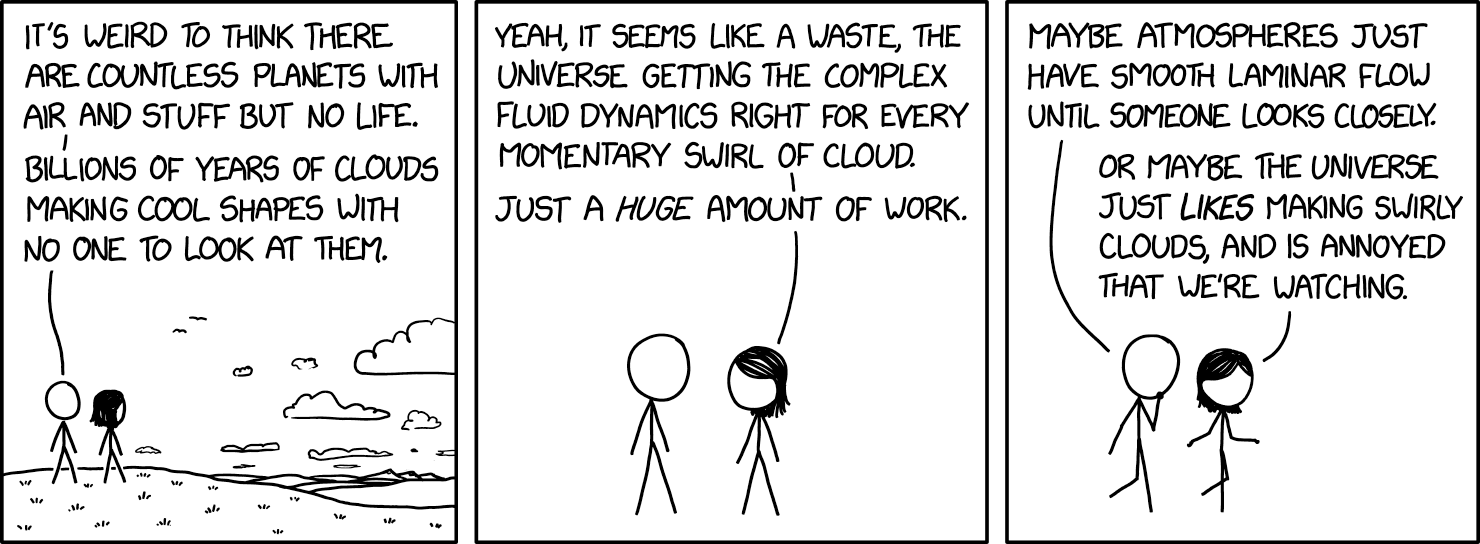
\includegraphics[width=\linewidth]{figures/cloud_swirls.png}

    {
        \footnotesize \color{gray}
        Randall Munroe, \href{https://xkcd.com/2664/}{xkcd.com}
    }
\end{center}
\vfill

\chapter*{Abstract}
Weather and climate models use so-called parametrisation schemes to emulate the
effects of small-scale processes that they cannot resolve explicitly.
Data-driven methods for constructing these schemes have attracted considerable
research attention in recent years, but remain subject to important outstanding
questions. Using the simpler case of two-dimensional \rb{} convection as an
analogue for the climate system, this thesis presents a complete proof of
concept for a data-driven approach that quantifies subgrid tendencies---the
effects of unresolvable processes---by systematically coarse-graining
high-resolution training data. A parametrisation scheme constructed using this
method is shown to be able to improve both the short-term forecast accuracy and
long-term statistical accuracy of a low-resolution model. This work identifies
and addresses subtle technicalities associated with the coarse-graining
process, establishing concrete computational tools with which future work will
be able to address remaining unanswered questions surrounding data-driven
methods and potentially inform parametrisation development in real
weather and climate models.


\tableofcontents

\makeatletter\@openrighttrue\makeatother
\mainmatter
\end{document}
